\documentclass[]{book}
\usepackage{lmodern}
\usepackage{amssymb,amsmath}
\usepackage{ifxetex,ifluatex}
\usepackage{fixltx2e} % provides \textsubscript
\ifnum 0\ifxetex 1\fi\ifluatex 1\fi=0 % if pdftex
  \usepackage[T1]{fontenc}
  \usepackage[utf8]{inputenc}
\else % if luatex or xelatex
  \ifxetex
    \usepackage{mathspec}
  \else
    \usepackage{fontspec}
  \fi
  \defaultfontfeatures{Ligatures=TeX,Scale=MatchLowercase}
\fi
% use upquote if available, for straight quotes in verbatim environments
\IfFileExists{upquote.sty}{\usepackage{upquote}}{}
% use microtype if available
\IfFileExists{microtype.sty}{%
\usepackage{microtype}
\UseMicrotypeSet[protrusion]{basicmath} % disable protrusion for tt fonts
}{}
\usepackage{hyperref}
\hypersetup{unicode=true,
            pdftitle={PA 5928},
            pdfauthor={Tao Tao},
            pdfborder={0 0 0},
            breaklinks=true}
\urlstyle{same}  % don't use monospace font for urls
\usepackage{natbib}
\bibliographystyle{apalike}
\usepackage{color}
\usepackage{fancyvrb}
\newcommand{\VerbBar}{|}
\newcommand{\VERB}{\Verb[commandchars=\\\{\}]}
\DefineVerbatimEnvironment{Highlighting}{Verbatim}{commandchars=\\\{\}}
% Add ',fontsize=\small' for more characters per line
\usepackage{framed}
\definecolor{shadecolor}{RGB}{248,248,248}
\newenvironment{Shaded}{\begin{snugshade}}{\end{snugshade}}
\newcommand{\AlertTok}[1]{\textcolor[rgb]{0.94,0.16,0.16}{#1}}
\newcommand{\AnnotationTok}[1]{\textcolor[rgb]{0.56,0.35,0.01}{\textbf{\textit{#1}}}}
\newcommand{\AttributeTok}[1]{\textcolor[rgb]{0.77,0.63,0.00}{#1}}
\newcommand{\BaseNTok}[1]{\textcolor[rgb]{0.00,0.00,0.81}{#1}}
\newcommand{\BuiltInTok}[1]{#1}
\newcommand{\CharTok}[1]{\textcolor[rgb]{0.31,0.60,0.02}{#1}}
\newcommand{\CommentTok}[1]{\textcolor[rgb]{0.56,0.35,0.01}{\textit{#1}}}
\newcommand{\CommentVarTok}[1]{\textcolor[rgb]{0.56,0.35,0.01}{\textbf{\textit{#1}}}}
\newcommand{\ConstantTok}[1]{\textcolor[rgb]{0.00,0.00,0.00}{#1}}
\newcommand{\ControlFlowTok}[1]{\textcolor[rgb]{0.13,0.29,0.53}{\textbf{#1}}}
\newcommand{\DataTypeTok}[1]{\textcolor[rgb]{0.13,0.29,0.53}{#1}}
\newcommand{\DecValTok}[1]{\textcolor[rgb]{0.00,0.00,0.81}{#1}}
\newcommand{\DocumentationTok}[1]{\textcolor[rgb]{0.56,0.35,0.01}{\textbf{\textit{#1}}}}
\newcommand{\ErrorTok}[1]{\textcolor[rgb]{0.64,0.00,0.00}{\textbf{#1}}}
\newcommand{\ExtensionTok}[1]{#1}
\newcommand{\FloatTok}[1]{\textcolor[rgb]{0.00,0.00,0.81}{#1}}
\newcommand{\FunctionTok}[1]{\textcolor[rgb]{0.00,0.00,0.00}{#1}}
\newcommand{\ImportTok}[1]{#1}
\newcommand{\InformationTok}[1]{\textcolor[rgb]{0.56,0.35,0.01}{\textbf{\textit{#1}}}}
\newcommand{\KeywordTok}[1]{\textcolor[rgb]{0.13,0.29,0.53}{\textbf{#1}}}
\newcommand{\NormalTok}[1]{#1}
\newcommand{\OperatorTok}[1]{\textcolor[rgb]{0.81,0.36,0.00}{\textbf{#1}}}
\newcommand{\OtherTok}[1]{\textcolor[rgb]{0.56,0.35,0.01}{#1}}
\newcommand{\PreprocessorTok}[1]{\textcolor[rgb]{0.56,0.35,0.01}{\textit{#1}}}
\newcommand{\RegionMarkerTok}[1]{#1}
\newcommand{\SpecialCharTok}[1]{\textcolor[rgb]{0.00,0.00,0.00}{#1}}
\newcommand{\SpecialStringTok}[1]{\textcolor[rgb]{0.31,0.60,0.02}{#1}}
\newcommand{\StringTok}[1]{\textcolor[rgb]{0.31,0.60,0.02}{#1}}
\newcommand{\VariableTok}[1]{\textcolor[rgb]{0.00,0.00,0.00}{#1}}
\newcommand{\VerbatimStringTok}[1]{\textcolor[rgb]{0.31,0.60,0.02}{#1}}
\newcommand{\WarningTok}[1]{\textcolor[rgb]{0.56,0.35,0.01}{\textbf{\textit{#1}}}}
\usepackage{longtable,booktabs}
\usepackage{graphicx,grffile}
\makeatletter
\def\maxwidth{\ifdim\Gin@nat@width>\linewidth\linewidth\else\Gin@nat@width\fi}
\def\maxheight{\ifdim\Gin@nat@height>\textheight\textheight\else\Gin@nat@height\fi}
\makeatother
% Scale images if necessary, so that they will not overflow the page
% margins by default, and it is still possible to overwrite the defaults
% using explicit options in \includegraphics[width, height, ...]{}
\setkeys{Gin}{width=\maxwidth,height=\maxheight,keepaspectratio}
\IfFileExists{parskip.sty}{%
\usepackage{parskip}
}{% else
\setlength{\parindent}{0pt}
\setlength{\parskip}{6pt plus 2pt minus 1pt}
}
\setlength{\emergencystretch}{3em}  % prevent overfull lines
\providecommand{\tightlist}{%
  \setlength{\itemsep}{0pt}\setlength{\parskip}{0pt}}
\setcounter{secnumdepth}{5}
% Redefines (sub)paragraphs to behave more like sections
\ifx\paragraph\undefined\else
\let\oldparagraph\paragraph
\renewcommand{\paragraph}[1]{\oldparagraph{#1}\mbox{}}
\fi
\ifx\subparagraph\undefined\else
\let\oldsubparagraph\subparagraph
\renewcommand{\subparagraph}[1]{\oldsubparagraph{#1}\mbox{}}
\fi

%%% Use protect on footnotes to avoid problems with footnotes in titles
\let\rmarkdownfootnote\footnote%
\def\footnote{\protect\rmarkdownfootnote}

%%% Change title format to be more compact
\usepackage{titling}

% Create subtitle command for use in maketitle
\providecommand{\subtitle}[1]{
  \posttitle{
    \begin{center}\large#1\end{center}
    }
}

\setlength{\droptitle}{-2em}

  \title{PA 5928}
    \pretitle{\vspace{\droptitle}\centering\huge}
  \posttitle{\par}
    \author{Tao Tao}
    \preauthor{\centering\large\emph}
  \postauthor{\par}
      \predate{\centering\large\emph}
  \postdate{\par}
    \date{2019-08-13}

\usepackage{booktabs}

\begin{document}
\maketitle

{
\setcounter{tocdepth}{1}
\tableofcontents
}
\hypertarget{prerequisites}{%
\chapter{Prerequisites}\label{prerequisites}}

This is a \emph{sample} book written in \textbf{Markdown}. You can use anything that Pandoc's Markdown supports, e.g., a math equation \(a^2 + b^2 = c^2\).

The \textbf{bookdown} package can be installed from CRAN or Github:

\begin{Shaded}
\begin{Highlighting}[]
\KeywordTok{install.packages}\NormalTok{(}\StringTok{"bookdown"}\NormalTok{)}
\CommentTok{# or the development version}
\CommentTok{# devtools::install_github("rstudio/bookdown")}
\end{Highlighting}
\end{Shaded}

Remember each Rmd file contains one and only one chapter, and a chapter is defined by the first-level heading \texttt{\#}.

To compile this example to PDF, you need XeLaTeX. You are recommended to install TinyTeX (which includes XeLaTeX): \url{https://yihui.name/tinytex/}.

\hypertarget{introduction-to-rstudio}{%
\chapter{Introduction to RStudio}\label{introduction-to-rstudio}}

\hypertarget{what-is-r}{%
\section{What is R}\label{what-is-r}}

\textbf{R} is a type of programming language and supports many tasks including statistical computation and grapics.

\hypertarget{what-is-r-studio}{%
\section{What is R Studio}\label{what-is-r-studio}}

\textbf{RStudio} is a programming software for editing and running R code.

\hypertarget{install-r-rstudio}{%
\section{Install R + RStudio}\label{install-r-rstudio}}

For better coding and running R, you should install both R and RStudio.You could only code R with the installation with R only, however, RStudio provides you with more conveinece during the working process. In this course, we will use RStudio to do all the course stuff. So please make sure you install both two!
R could be downloaded \href{https://www.r-project.org/}{here} and RStudio could be downloaded \href{https://www.rstudio.com/products/rstudio/download/}{here}.

\hypertarget{familiar-with-the-user-interface-of-r-studio}{%
\section{Familiar with the user interface of R Studio}\label{familiar-with-the-user-interface-of-r-studio}}

Below is the figure showing a screenshot of the user interface of RStudio. You will find couple of panes/windows with different usages.

\begin{enumerate}
\def\labelenumi{\arabic{enumi}.}
\tightlist
\item
  \textbf{Manu/Tool Bar}
\item
  \textbf{Source} The pane where you write and edit your code.
\item
  \textbf{Environment/History} Environment lists all the variables that you are using. History presents the codes you have runned before.
\item
  \textbf{Console} Console is original R interactive window. You could input codes and see the results here.
\item
  \textbf{Plots/Help} Plots window shows the output figures. Help windows presents the information of the function or package you check.
\end{enumerate}

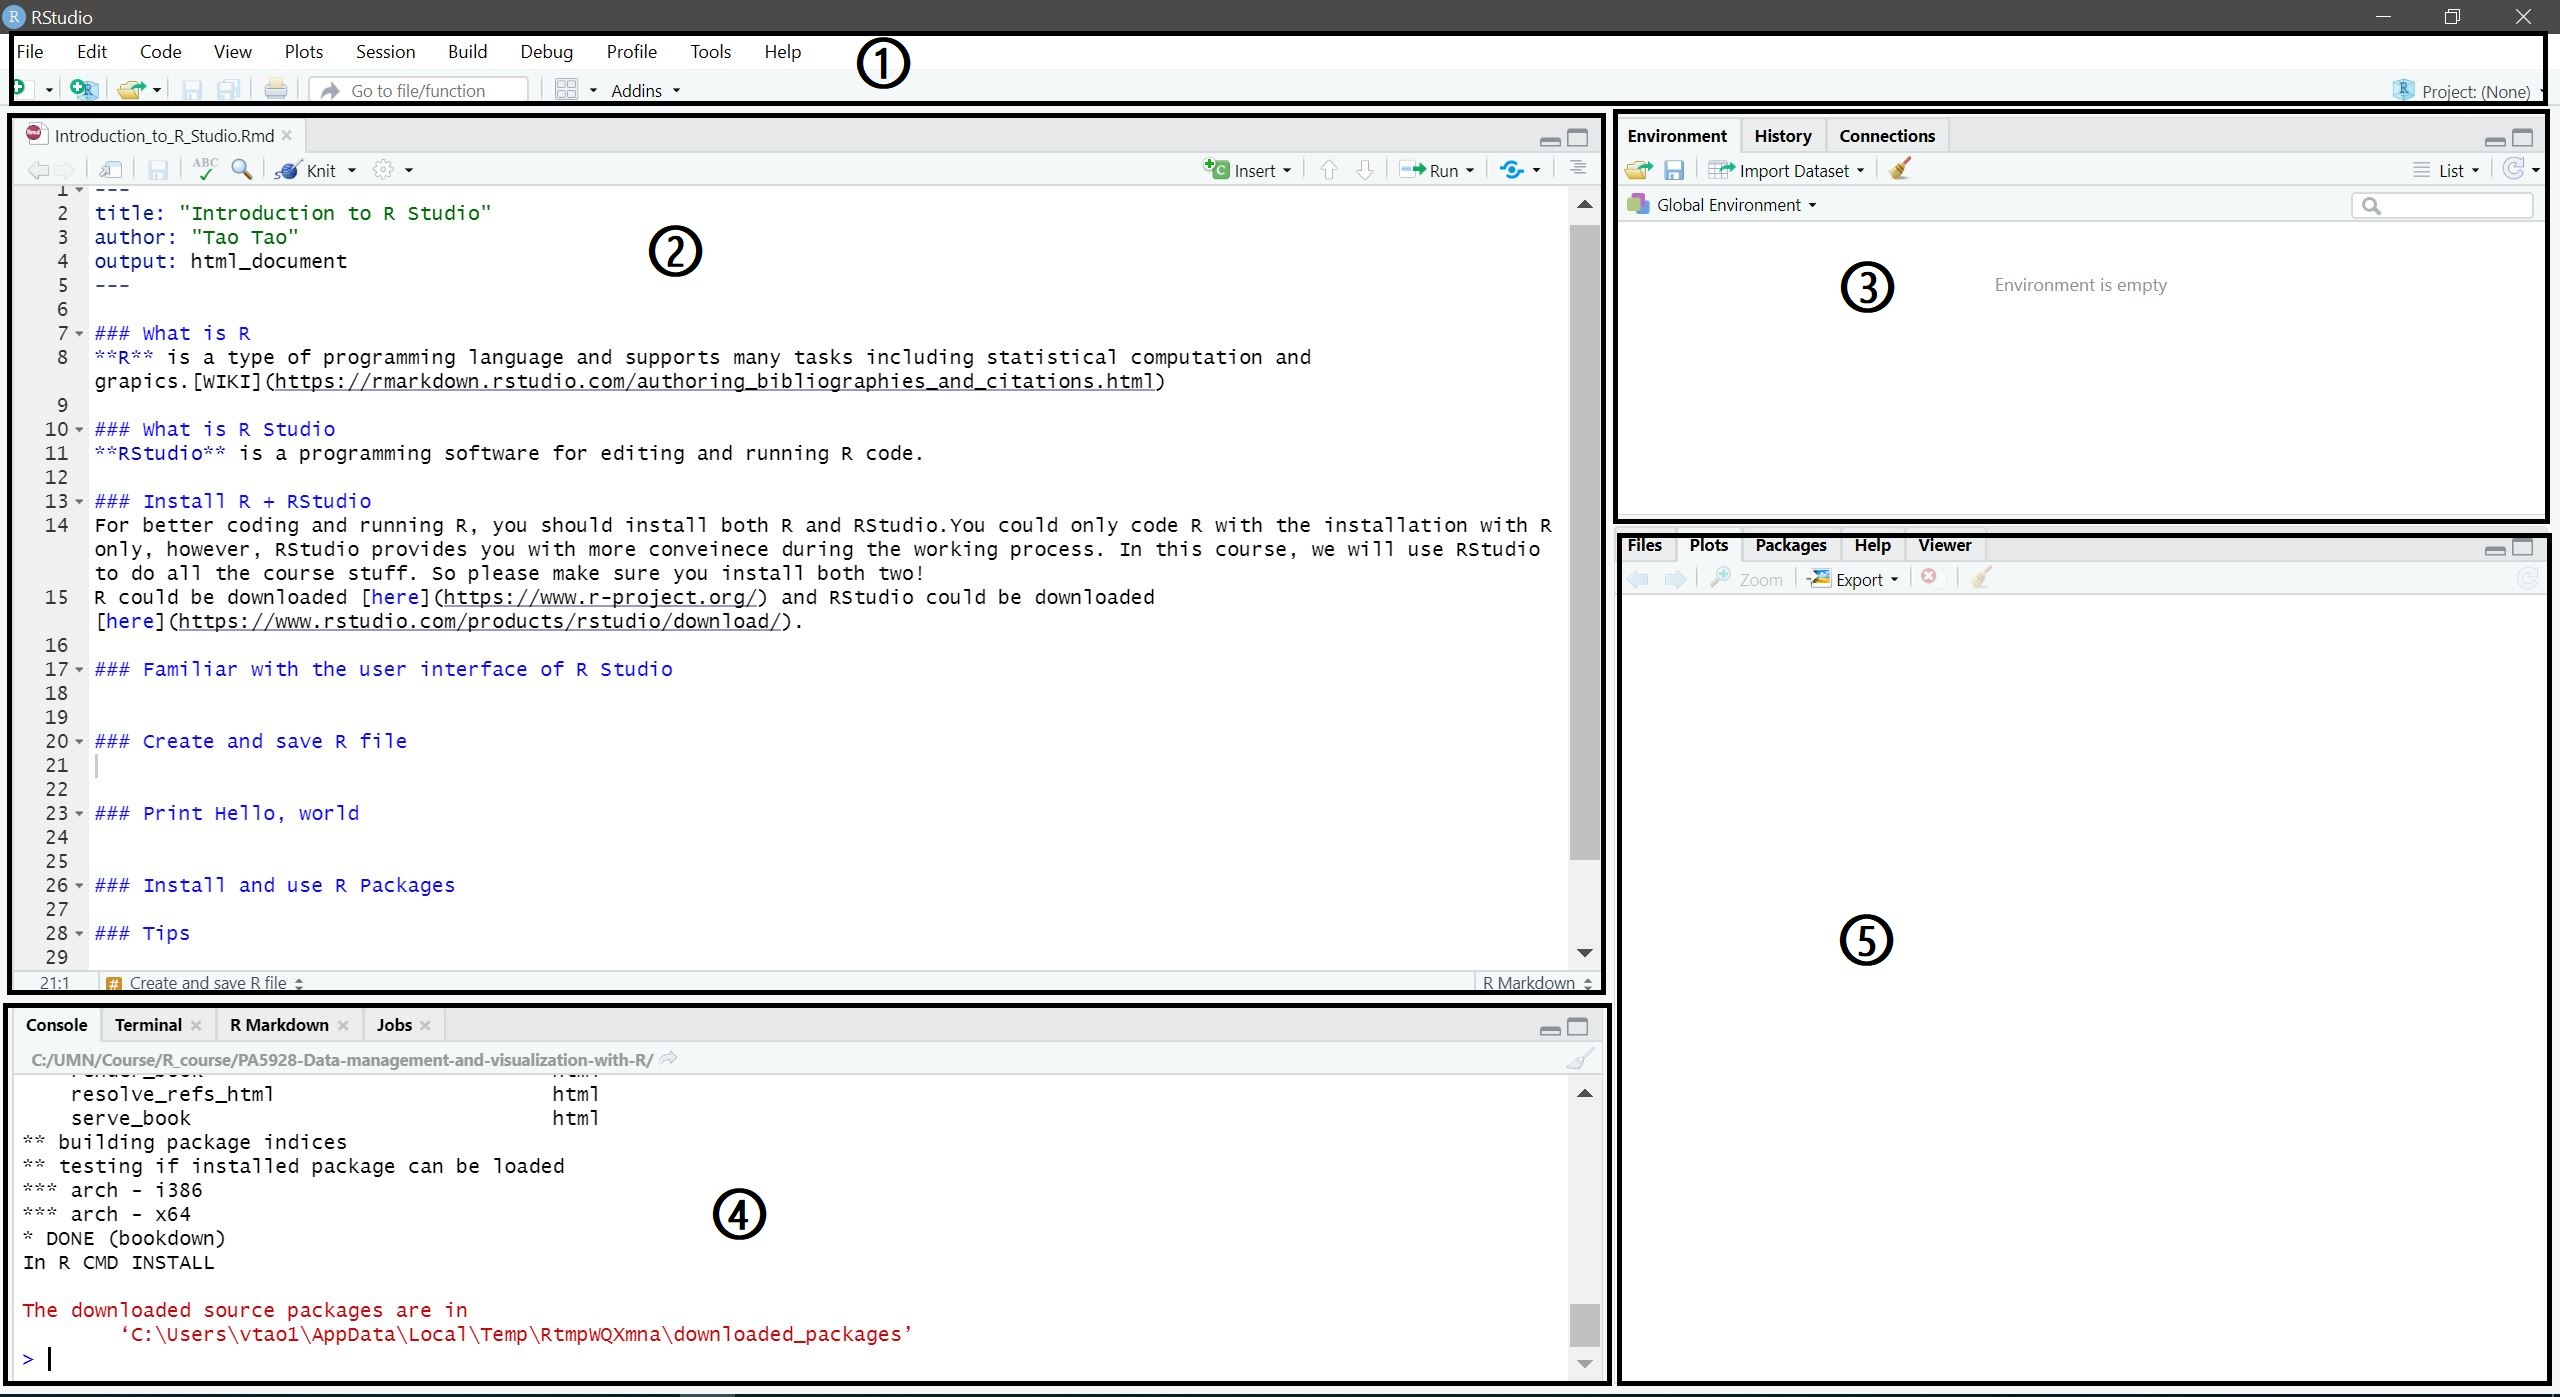
\includegraphics{Pics/RStudio.JPG}

\hypertarget{create-and-save-r-file}{%
\section{Create and save R file}\label{create-and-save-r-file}}

Three ways to create a R file in the RStudio:

\begin{verbatim}
1. Manu -> File -> New File -> R Script
2. Shortcut: Ctrl + Shift + N
3. Tool Bar -> New file button
\end{verbatim}

Also three ways to save R file

\begin{verbatim}
1. Manu -> File -> Save
2. Shortcut: Ctrl + S
3. Tool Bar -> Save file button
\end{verbatim}

\hypertarget{print-hello-world}{%
\section{Print Hello, world}\label{print-hello-world}}

Now, let's try to input some codes and run them! Let's let R print the very classic ``Hello, world!'' with \texttt{print()} function.
We could run the codes in several ways:

\begin{enumerate}
\def\labelenumi{\arabic{enumi}.}
\tightlist
\item
  Select the codes or put the cursor in the line of your code, and click the Run button located in the right-top position of the console pane.
\item
  Select the codes or put the cursor in the line of your code, and use shortcut: Ctrl + Enter
\item
  You could also click the Re-run button near the Run button to re-run the codes you runned last time
\end{enumerate}

\begin{Shaded}
\begin{Highlighting}[]
\KeywordTok{print}\NormalTok{(}\StringTok{'Hello, world!'}\NormalTok{)}
\end{Highlighting}
\end{Shaded}

\begin{verbatim}
## [1] "Hello, world!"
\end{verbatim}

Because what we need to output here is a \textbf{string varible}, we have to put them in the quotation mark. Either single quotation or double quotation mark works well. Let's see another example.

\begin{Shaded}
\begin{Highlighting}[]
\KeywordTok{print}\NormalTok{(}\DecValTok{5928}\NormalTok{)}
\end{Highlighting}
\end{Shaded}

\begin{verbatim}
## [1] 5928
\end{verbatim}

Here, 5928 is an integer and we do not need to put them in the quotation mark.

\hypertarget{install-and-use-r-packages}{%
\section{Install and use R Packages}\label{install-and-use-r-packages}}

R is easy to use because it has many packages with different usages. These packages could help you acomplish some complex tasks with several lines of codes.
Some packages have been already been installed and you could use them directly. However, most of the packages have to be installed before you want to use them. There are couple of ways you could install a package. Let's take the \texttt{gbm} package for example.

\begin{verbatim}
1. Manu -> Tools -> Install Packages... -> Input the package name -> Click Install button
\end{verbatim}

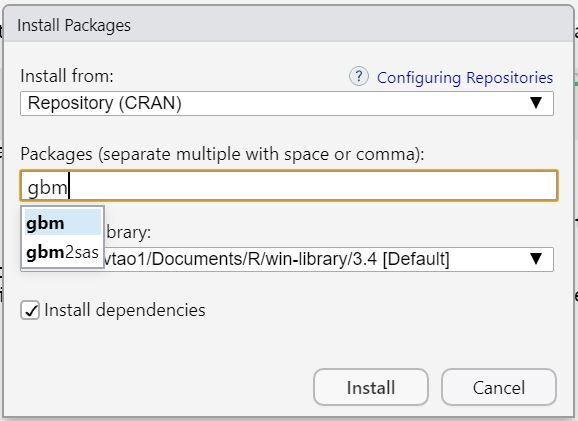
\includegraphics[width=0.35\textwidth,height=\textheight]{Pics/InstallPackages.JPG}

\begin{verbatim}
2. Use the code below:
install.packages("gbm")
\end{verbatim}

After the installation of the package, you have import the it with \texttt{library()} function before you use the functions in it.

\begin{Shaded}
\begin{Highlighting}[]
\KeywordTok{library}\NormalTok{(gbm)}
\end{Highlighting}
\end{Shaded}

We will spend more time in the future classes to explore the various R packages and their different usages.

\hypertarget{make-notes}{%
\section{Make notes}\label{make-notes}}

It is important to write notes for your codes. It could help others or even yourself understand your codes easily. Use hash tag to indicate the notes. For example,

\begin{Shaded}
\begin{Highlighting}[]
\NormalTok{gbm1 <-}\StringTok{ }\KeywordTok{gbm}\NormalTok{(AvgMet}\OperatorTok{~}\NormalTok{PkAreaH}\OperatorTok{+}\NormalTok{StpNumH}\OperatorTok{+}\NormalTok{DisToMin,  }\CommentTok{# formula}
            \DataTypeTok{data=}\NormalTok{MetM,                        }\CommentTok{# dataset  }
            \DataTypeTok{var.monotone=}\KeywordTok{c}\NormalTok{(}\OperatorTok{+}\DecValTok{1}\NormalTok{, }\KeywordTok{rep}\NormalTok{(}\DecValTok{0}\NormalTok{,}\DecValTok{10}\NormalTok{),}\KeywordTok{rep}\NormalTok{(}\DecValTok{0}\NormalTok{,}\DecValTok{15}\NormalTok{)), }
            \DataTypeTok{distribution=}\StringTok{"gaussian"}\NormalTok{,          }\CommentTok{# see the help for other choices  }
            \DataTypeTok{n.trees=}\DecValTok{5000}\NormalTok{,                     }\CommentTok{# number of trees  }
            \DataTypeTok{shrinkage=}\FloatTok{0.001}\NormalTok{,                  }\CommentTok{# shrinkage or learning rate, 0.001 to 0.1 usually work  }
            \DataTypeTok{interaction.depth=}\DecValTok{6}\NormalTok{,              }\CommentTok{# 1: additive model, 2: two-way interactions, etc.  }
            \DataTypeTok{bag.fraction =} \FloatTok{0.5}\NormalTok{,               }\CommentTok{# subsampling fraction, 0.5 is probably best  }
            \DataTypeTok{n.minobsinnode =} \DecValTok{10}\NormalTok{,              }\CommentTok{# minimum total weight needed in each node}
            \DataTypeTok{cv.folds =} \DecValTok{5}\NormalTok{)}
\end{Highlighting}
\end{Shaded}

R will not run the codes after hash tags in each line.

Please try to write simple but necessary notes for the codes. Keep this as a good habbit and you will thank yourself in the future.

\hypertarget{tips-updating}{%
\section{Tips (Updating)}\label{tips-updating}}

\begin{enumerate}
\def\labelenumi{\arabic{enumi}.}
\tightlist
\item
  You could divide your codes into sections by interting chunks before each sections with the shortcut: Ctrl + Shift + R. This will help you organize your codes.
\end{enumerate}

\hypertarget{reference}{%
\section{Reference}\label{reference}}

\begin{enumerate}
\def\labelenumi{\arabic{enumi}.}
\tightlist
\item
  \href{https://datascienceplus.com/introduction-to-rstudio/}{Introduction to RStudio}
\end{enumerate}

\bibliography{book.bib,packages.bib}


\end{document}
